%! TEX root = ../main.tex
\chapter[TIC's en la Educación]{Tecnologías de la Información y Comunicación en
    la Educación}
\label{chap:tics}

\observacion{Enfocar desde un marco común (tendencias)}

Las \Gls{tic} son un conjunto de herramientas tecnológicas y recursos utilizados
para comunicar, crear, diseminar, almacenar y manejar la
información\cite{unesco:ict}. Estas tecnologías abarcan computadoras personales,
internet, radio, televisión y telefonía\cite{tinio:ict}.

Las \Gls{tic} fueron utilizadas como complemento a la educación desde los
inicios de la misma con la radio y la televisión. Fueron vistas como un
complemento a las herramientas utilizadas en clase, como complemento del libro,
o como una herramienta que elimina la distancia física entre el profesor y el
alumno\cite{unesco:ict}. 

A continuación se describe en detalle la relación de las  \Gls{tic} con la
educación, explicando las corrientes pedagógicas conocidas como instruccionismo
y construccionismo para detallar la relación de las mismas con la tecnología
como herramienta de apoyo.

%! TEX root = ../main.tex
\section{Educación Tradicional}

La educación tradicional o instruccionismo se basa en la transferencia de 
conocimiento del profesor al alumno, se enfoca más en el profesor, en la 
capacidad del mismo, y en el producto final como resultado de un proceso 
no interactivo y bien documentado\cite{igi:instructionism}. Los mecanismos 
tradicionales para probar la efectividad de este tipo de enseñanza son los exámenes.

%\fixme{La educación tradicional o instruccionismo se basa en el concepto de que
%   existe un profesor y un alumno. El profesor transfiere el conocimiento que
%    ha adquirido de diferentes métodos (educación, experiencia, etc) a un alumno
%    que es un receptor pasivo de información }{No copy/paste en la
%    intro}\cite{johnson2005instructionism}.

%Se enfoca más en el profesor, y en la enseñanza, y en el producto final como
%resultado de un proceso no interactivo y bien
%documentado\cite{igi:instructionism}. Los mecanismos tradicionales para poder
%probar la efectividad de este tipo de enseñanza son los exámenes.

%\fixme{La principal}{Ablandar} critica a este modelo es que se enfoca la
%enseñanza y no el aprendizaje, mientras más se enseña, más se aprende.
%\textbf{Esto contradice al sentido común en el sentido de que, cosas básicas
%    como caminar o hablar, aprendemos sin la necesidad de un
%    profesor\cite{ackoff:education}\cite{johnson2005instructionism}.}{Más
%    énfasis en el aprender haciendo y usar referencias, no ``el sentido común''}

Una de las principales criticas a este modelo de enseñanza por parte de las
demás corrientes pedagógicas es que según ellas el instruccionismo se basa en la
idea de que  \enquote{cuanto mas se enseña mas se aprende} y esto contradice al
enfoque de \enquote{aprender haciendo} teniendo en cuenta que cosas como caminar
o hablar se aprende sin la necesidad de un profesor
\cite{ackoff:education,johnson2005instructionism}. 

%Tradicionalmente el rol de las TIC's en la educación se vio relegada a la de
%sustituto del libro y/o de presentaciones en clase, es decir, es un mecanismo
%más para trasmitir el conocimiento del maestro al alumno.


%! TEX root = ../main.tex
\section[Educación con TIC's]{Educación con las Tecnologías de la Información y
    Comunicación}
\label{sec:tics_educacion}

Las expectativas iniciales acerca del impacto de las \Gls{tic} en la educación
fueron ampliamente superiores a los resultados obtenidos\cite{unesco:ict}. Con
el advenimiento de las computadoras se redujo esta diferencia entre las
expectativas  y lo obtenido, en mayor medida por que se utilizo a las \Gls{tic}
en conjunto con  tecnologías como Internet, y los efectos positivos en la
educación fueron aumentando gradualmente\cite{unesco:ict}.

Una de las principales ventajas de la utilización de las \Gls{tic} en la
educación es su aplicabilidad en áreas como:

\begin{itemize}

\item \textbf{Nuevos modelos pedagógicos:} teorías como el constructivismo moderno
    enfatizan el proceso de como adquirir (aprendizaje) conocimiento y no
    solamente como transmitir el conocimiento en sí (enseñanza).

\item \textbf{Eliminación de distancias:} Con la aparición de las computadoras y los
    satélites,  el mundo se ha convertido en una aldea global, y las distancias
    en cuestiones de transmisión de información se han vuelto
    insignificantes\cite{mohammed2013information},  los medios tradicionales
    como bibliotecas, o escuelas están limitados a un espacio  físico, con el
    uso de las \Gls{tic}, esta restricción física desaparece\cite{tinio:ict}.

\item \textbf{Colaboración distribuida:} como consecuencia del punto anterior, los
    alumnos pueden colaborar de manera más sencilla pues no tienen limitaciones
    físicas. Además, los alumnos pueden consultar con expertos que están en
    linea, e incluso tener mentores en linea, estas tutorías pueden ser uno a
    uno, por ejemplo mediante comunicaciones por correo electrónico. Además
    permite la colaboración masiva entre estudiantes de intereses comunes,
    mediante foros y redes sociales\cite{unesco:ict}.

\item \textbf{Motivación para aprender:} Las \Gls{tic} tienen un impacto positivo en el
    proceso de aprendizaje especialmente en lo referente al compromiso
    con\cite{passey2004motivational,egenfeldt2007third}:
	    
    \begin{itemize}
    \item La actividad: a través de estímulos visuales, auditivos, etc.
    \item La capacidad de investigación: es más fácil acceder a gran cantidad de
        información bibliográfica.
    \item La capacidad de escritura y lectura: emitiendo compartir  ideas de
        manera más legible y mejorarlas iterativamente.
    \item La capacidad de presentación: es más fácil presentar trabajos
        profesionalmente a un público mayor.
    \end{itemize}
	    
\item \textbf{Adquisición de habilidades básicas:} las habilidades necesarias para
    utilizar de manera efectiva las \Gls{tic} se están convirtiendo en una
    necesidad básica, un aprendizaje guiado por las mismas puede ayudar a una
    rápida asimilación de los conceptos \fixme{relacionados}{Por qué?}.

\end{itemize}

Uno de los desafíos más importantes que enfrentan las \Gls{tic} para convertirse
en una alternativa viable es la inversión en infraestructura
necesaria\cite{unesco:ict}.

\subsection{Evolución}

La historia de las \Gls{tic} en educación comienza en la \enquote{Open
    University of United Kingdom} que en $1969$ se establece como la primera
institución educativa dedicada a la enseñanza a distancia utilizando las, para
aquel entonces, nuevas tecnologías\cite{tinio:ict}. 

El análisis de la historia de las \Gls{tic} en educación es indispensable,
aunque existe una corriente que tiende a desestimar las experiencias pasadas,
cuyo principal fundamente es la velocidad con la que la tecnología evoluciona,
es importante el estudio de la evolución de la misma pues los errores
pedagógicos cometidos, aunque puedan parecer evidentes hoy en día, condujeron a
nuevos modelos y conclusiones que son la base de la utilización de las \Gls{tic}
hoy en día\cite{mcdougall2006theory}.

El impacto de las \Gls{tic} en la educación no ha sido constante durante su
historia, sino más bien, ha evolucionado de ser un medio más de traspaso de
información, hasta hoy en día, donde permite generar
conocimiento\cite{tinio:ict}.

\begin{figure}
    \centering
    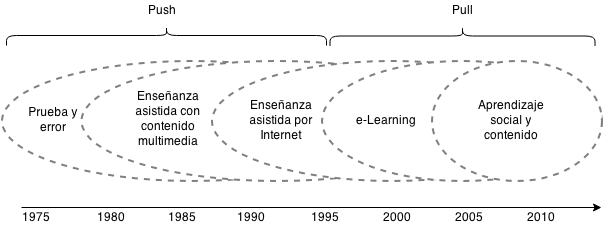
\includegraphics[scale=0.75]{tics/images/tics_history.png}
    \caption{Utilización de las \Gls{tic} en la educación desde el año $1975$}
    \label{fig:history_tics}
\end{figure}

Para entender la historia de las \Gls{tic} en la educación, se presenta el
gráfico~\ref{fig:history_tics}, en el cual se observa la evolución que sufrió la
utilización de las \Gls{tic} como herramienta en la educación. Se observa que se
parte la historia en cinco corrientes definidas, y a la vez, estas corrientes se
agrupan según el mecanismo de obtención de información, las tres primeras
corrientes se denominan \textit{pull} y las siguientes dos se denominan
\textit{push}. \textit{Pull} se refiere a que los estudiantes obtenían la
información sin participar en la creación de la misma, y \textit{push} es cuando
los alumnos son creados activos de conocimiento\cite{white:ict,leinonen:ict}.

Aunque la figura~\ref{fig:history_tics} muestre un progreso lineal de las
corrientes, este progreso no es igual en todo el mundo, y la el grado de impacto
de las \Gls{tic} varia entre países, lo que se conoce como una brecha
tecnológica. Las fechas utilizadas en el figura~\ref{fig:history_tics} son
relacionadas a la evolución en los Estados Unidos de Norte America.

\subsubsection{Pull}

A finales de la década de $1970$ e inicios de la década de $1980$,  la
complejidad técnica de las computadoras limitaba la cantidad de herramientas
disponibles, los programas eran desarrollados por profesores, y su objetivo era
que los alumnos puedan poner en práctica lo aprendido en el aula. El campo de
aplicación de las herramientas se limitaban a matemáticas y lenguaje, donde se
podía evaluar inmediatamente los resultados proveídos por los alumnos, pues,
normalmente era un enunciado y una lista posible de opciones. La cantidad
limitada de opciones para responder, provocó que los alumnos no interpreten los
resultados, sino prueben todas las posibles opciones hasta pasar al siguiente
enunciado, sin realizar ningún aprendizaje significativo\cite{leinonen:ict},
este tipo de juegos se denomina \enquote{Prueba y Error}.

Cuando aparecieron en el mercado computadoras con multimedia, a finales de la
década de $1980$, la utilización de las \Gls{tic} se simplificaron y dieron
contenido a la posibilidad de incluir contenido multimedia, se argumentó que los
ejercicios de tipo \enquote{Prueba y Error} no cumplieron su objetivo de una
educación profunda por que no contenían multimedia\cite{leinonen:ict}, así, en
se empezaron a distribuir las aplicaciones eran distribuidas por
\textit{CD-ROM}, se actualizaban de manera frecuente, y podían contener gran
cantidad de contenido multimedia.

Con la creación de los juegos del tipo \enquote{Prueba y Error} y el contenido
multimedia, se inicio a un nueva corriente denominada \emph{Edutainment},
palabra que representa la unión de la educación y el entretenimiento. Así el
\emph{edutainment} pretende agregar entretenimiento a la educación, se ve al
alumno como un receptor pasivo de información que debe asimilarla, y para
aumentar la implicación de los alumnos, el entretenimiento era
agregado\cite{resnick:2004}.

Los \emph{edutainment} se basan principalmente en el conductismo y el
cognoscitivismo, se enfoca en juegos sencillos que transmiten información simple
al usuario, su estructura se basa en un objetivo claro que está separado de la
experiencia educativa\cite{egenfeldt2007third}. 

\emph{Math Blaster} (ver~\ref{fig:math_blaster}) es un \emph{edutainment} donde
el alumno debe responder repetitivamente preguntas aritméticas para obtener
municiones, luego con esas municiones debe completar diferentes misiones en una
nave\cite{bruckman1999can}. Como todas las preguntas se responden mediante un
mecanismo de selección múltiple, y no existe penalización por fallar una
respuesta, los alumnos no reflexionan sobre las respuestas elegidas, seleccionan
una opción aleatoria y si no es la correcta, prueban otra, tras una cantidad
finita de intentos, siempre se obtiene la recompensa deseada.

\begin{figure}[ht!] 
\centering 
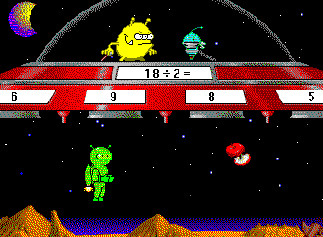
\includegraphics[scale=0.5,natwidth=296,natheight=217]{tics/images/math_blaster.jpg}
\caption{Math Blaster, \emph{edutainment} del año 1987}
\label{fig:math_blaster} 
\end{figure}

\begin{figure}[ht!] 
\centering 
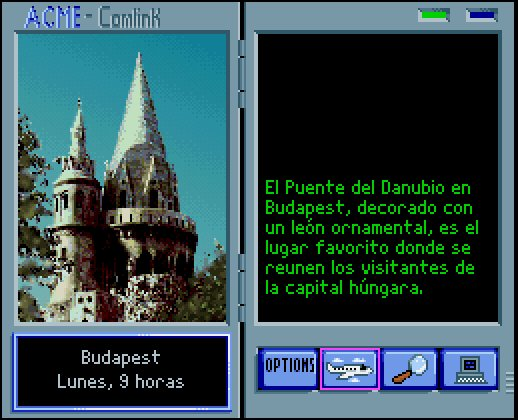
\includegraphics[scale=0.5]{tics/images/carmen.jpg}
\caption{Donde en el mundo esta Carmen Sandiego} 
\label{fig:carmen}
\end{figure}

\enquote{Donde en el mundo esta Carmen Sandiego} (ver~\ref{fig:carmen}) es un
juego que representa el potencial multimedia de esta época, el objetivo del
juego era detener a una serie de criminales mediante una serie de pistas que
eran provistas en forma de texto. Este exitoso juego demuestra las falencias de
esta época, siendo visualmente muy atractivo, y con contenido multimedia acorde
a su tiempo, no era más que \emph{prueba y error}, cada nivel del juego podía
ser completado sin leer la información proveída educativa\cite{charsky:2010}.

Los \emph{edutainment} no logran enseñar habilidades complejas, se enfocan
principalmente en enseñar tareas extremadamente repetitivas que no dependen de
un contexto\cite{charsky:2010,egenfeldt2007third,bruckman1999can}, son
excelentes para enseñar a sumar, pero no para aplicar ese conocimiento, analizar
y obtener conclusiones, o evaluar lo que aprendieron.

Las principales causas por del fracaso de los \emph{edutainment} en su intento
de ser una alternativa viable a la educación son según\cite{egenfeldt2007third}: 

\begin{itemize}

\item \textbf{Falta de motivación interna:} los \emph{edutainment} se centran en
    motivaciones externas, y dejan de lado la motivación interna. Se centran en
    dar recompensas por acciones lo que es una motivación externa, que en que el
    alumno se sienta emocionado al finalizar un nivel, lo que es una forma de
    motivación interna.

\item \textbf{Aprendizaje como anexo:} el principal objetivo del desarrollo de un
    \emph{edutainment} es el de entretener, los objetivos pedagógicos son
    agregados al final. Adicionalmente, este aprendizaje se provee a través de
    largos textos que normalmente son omitidos.

\item \textbf{Interacción limitada:} son construidos con una jugabilidad pobre,
    sin la posibilidad de realizar multiples acciones, normalmente limitados a
    seleccionar respuestas o moverse en un pequeño mundo. 

\item \textbf{Ejercicios de prueba y error sistemáticos:} todas las debilidades
    anteriores se pueden fundamentar en el hecho de que los juegos permiten al
    alumno intentar varias veces sin ser penalizados, además
    de que los alumnos no están motivados, provocaba que todas las opciones sean
    probadas sin el proceso de reflexión necesario para aprender, por ejemplo,
    varios juegos aritméticos solicitaban pruebas del tipo $2+2$ donde el alumno
    probaba diferentes resultados y luego memorizaba el mismo. Se enseñaba a
    probar opciones sin sentido antes que entender y analizar la experiencia.

\end{itemize}

Los \emph{edutainment} se limitan a enseñar tareas mecánicas, sin entender el
contexto en el que se aplican y por qué se realizan\cite{egenfeldt2007third}.

El contenido distribuido, aunque contribuyo a la calidad del contenido proveído,
no resolvió el problema de contenido actualizado, pues a comienzos de la década
de $1990$, con la popularización de Internet\footnote{Internet se concibió lo
    que hoy se conoce como \emph{World Wide Web}\cite{white:ict}, pero se
    masifico en la década de $1990$\cite{leinonen:ict}}, se genera más contenido
que el que puede ser distribuido por medios físicos, así se accede al tercer
hito de la figura~\ref{fig:history_tics}, donde el contenido es distribuido por
internet.

Las bases pedagógicas de los \emph{Edutainment} siguen siendo las mismas, la
incursión de internet solo permite contenido actualizado, los problemas
persisten y se crean nuevos factores que incrementan la brecha tecnológica,
ahora, además de poseer una computadora, es necesaria una conexión permanente.
La velocidad inicial de internet no es suficiente para proveer los mismos
entornos ricos en multimedia que sí lo proveían los CD-ROM\cite{leinonen:ict}.

Así se crea una nueva generación de \emph{edutainment}, que son distribuidos por
internet, actualizados constantemente, pero con los mismos problemas
\cite{leinonen:ict}.

Un cambio de paradigma permite poner fin a la época de los \emph{Pull}, se pone
especial énfasis en el aprendiz y no en el contenido, así se inicia la época
\emph{Push}.

\subsubsection{Push}

Se inicia con el \emph{E-Learning}, \emph{E-Learning} se define como la
educación y capacitación a través de medios digitales, incluye todo tipo de
medio capaz de distribuir información, puede ser de en tiempo real como
salas de conversaciones y videoconferencias o puede ser diferido, como por
ejemplo foros, enciclopedias. Es particularmente útil para educación a distancia
y con horarios flexibles. Se originó a finales de la década de $1990$ y tuvo su
apogeo a mediados de la década del $2000$, apoyada por la gran penetración de
las \Gls{tic} en la población\cite{punie:ict}.

Se distribuye contenido masivamente a los alumnos, y luego, de manera discreta
se permite a los mismos colaborar, dejando siempre en claro que primero se debe
asimilar toda la información posible y luego relacionarse con los
demás\cite{leinonen:ict}, esto evidencia algunos problemas pedagógicos heredados
de la época \emph{Pull}.


\begin{figure}[h] 
\centering 
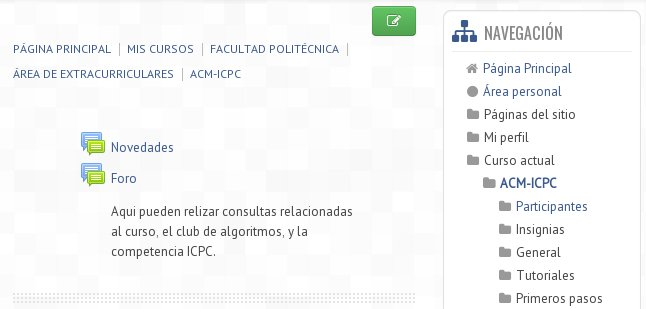
\includegraphics[scale=0.5]{tics/images/moodle.jpg}
\caption{Moodle, plataforma de e Learning} 
\label{fig:moodle}
\end{figure}


La plataforma \emph{Moodle} (ver~\ref{fig:moodle}) cuya primera versión salió en
el $2002$, es una de las principales herramientas del \emph{e-Learning} hoy en
día, permite la creación de cursos específicos por materia y sitios
especializados por instituciones académicas\cite{perkins2006using}. 

La utilización del \emph{e-Learning} tiene varios grados de aplicación en
entornos reales\cite{punie:ict}, que van desde ser simples elementos
complementarios a la clase, como por ejemplo un repositorio para las
diapositivas y otros materiales de clase, hasta cursos completamente en línea,
donde la clase ha sido completamente sustituida.

Sí bien, el \emph{e-Learning} permite la distribución y colaboración en
distintos niveles, no hace un enfoque en el aspecto pedagógico, y se centra en
la forma de transmitir información, y no como la recibe el
alumno\cite{leinonen:ict}.

Ideas que surgieron en la época \emph{Pull} son tomadas en cuenta a la hora de
diseñar nuevos esquemas de educación\cite{mcdougall2006theory}, las teorías del
construccionismo de \textit{Papert}, permiten enfocarse en el alumno, además del
ambiente en el que ocurre el aprendizaje\cite{egenfeldt2007third}.


\section{Problemas actuales}
\label{tics:problemas}

Durante la historia de las \Gls{tic} en la educación, se han encontrado
diferentes dificultades a la hora de aplicar los nuevos conceptos en la
educación, desde los primeros enfoques que carecían de bases pedagógicas válidas
hasta la actualidad.

El principal problema es falta de motivación de los profesionales de la
educación para emplear las \Gls{tic}\cite{punie:ict}\cite{ict:romeo}.

El contenido proveído actualmente puede ser considerado como un conjunto de
buenas prácticas\cite{punie:ict} y así, omiten completa o parcialmente el
contexto donde esa buena práctica fue generado.

A la hora de educar a los educadores en la utilización de las \Gls{tic} no se
debe medir medidas cuantitavias, como las notas o el número de cursos, sino más
bien el impacto cualitativo de la educación

Las \Gls{tic} han tenido un impacto positivo en la educación\cite{punie:ict},
pero no han obtenido el impacto esperado.

Iniciativas como el \emph{Edutainment}, prometían ser la solución a los
problemas educacionales, sin embargo, su implementación no cumplio con las
expectativas, obtuvieron una reputación negativa, y hoy en día son considerados
como el peor tipo de educación, pues son un ejercicio de \emph{prueba-error}
ocultos bajo un juego poco entretenido\cite{resnick:2004}. La principal critica
contra los \emph{Edutainment} es su incapacidad de enseñar como aplicar
conceptos aprendidos a un entorno real\cite{resnick:2004}.

Mientras que la utilización de las \Gls{tic} puede eliminar problemas actuales
como el aislamiento y la falta de pensamiento de alto nivel\cite{punie:ict}, la
brecha social existente implica otro riesgo para la utilización de las \Gls{tic}
en la educación, aquellos que no posean los recursos económicos necesarios para
acceder a la misma no se verán beneficiados por las \Gls{tic}\cite{punie:ict}.



\section{Construccionismo y las TIC}

El construccionismo utiliza la tecnología como medio cognitivo  a diferencia de
la educación tradicional que la utiliza para la entrega de contenido. 

El construccionismo es un alternativa prometedora a la educación
tradicional.Desde el punto de vista tecnológico, el contruccionismo es ideal
pues el mismo requiere un alto dinamismo en el traspaso del conocimiento
\cite{sasha:construtivism}. 

El contruccionismo y las \Gls{tic} siempre han estado relacionados, ya que el
mismo se origino con un lenguaje de programación(LOGO)\cite{ict:ttc}. Un
característica importante de esta relación es que tienen la capacidad de
eliminar los problemas de distancia\cite{mariluz:seiousgames}.


\subsection{Historia}

Seymour Papert adoptó el término construccionismo en la década de 1980 para
representar una método pedagógico practicado por John Dewey a principios del
siglo 20. Este método buscaba que la responsabilidad de aprender recaiga en el
estudiante. 

Papert trabajó directamente con el psicólogo evolutivo y filósofo suizo Jean
Piaget, quién elaboro sus teorías de la educación y construcción del
conocimiento al ver e interactuar con los niños. A partir de esta observación
nació el constructivismo según el cual el conocimiento debe ser construido por
el estudiante y los nuevos significados deben ser obtenidos relacionándolos con
significados anteriores por los mismos estudiantes haciendo uso así de sus
propios sistemas de relaciones.

El construccionismo se diferencia de lo anterior en que los estudiantes
construyen las ideas o partes del mundo utilizando herramientas. La elaboración
de representaciones mentales mediante la construcción y el intercambio es la
metáfora del marco contruccionista. 

Durante 1980, Seymor Papert, Wally Feurzeig, Marvin Minsky y John McCarthy y los
miembros del Departamento de Inteligencia Artificial del \Gls{mit} y una
compañía de tecnología en Cambridge, Massachusetts, desarrollaron un nuevo
lenguaje de programación llamado LOGO que tenía por objeto que los estudiantes
construyeran sus modelos en notación LOGO\@. Este juego introduciría de forma
natural las ideas de los procedimientos, funciones, variables, recursividad, la
modularidad, entre otros.

La creación del lenguaje de programación LOGO dio inicio al construccionismo.

Los desarrolladores de LOGO alentaron el uso de la tecnología para la promoción
de nuevas formas de aprendizaje diferentes a las tradicionales. Las comunidades
que adoptaron al contruccionismo con la creación del lenguaje LOGO fueron en su
mayoría aquellas integradas por ingenieros informáticos y matemáticos
\cite{historia:2014}.

\subsection{Bases Pedagógicas}

Para el construccionismo, el conocimiento es construido por el estudiante en
lugar de ser trasmitido por el profesor\cite{moses:2003} y esto sucede
particularmente cuando el mismo se compromete en la elaboración de un producto o
artefacto que tenga un significado y pueda ser compartido\cite{valdivia:sg}. De
esta manera, se permite a los estudiantes elaborar sus propias interpretaciones
razonadas del mundo mediante la interacción con el mismo.

Según Papert, los alumnos estarán mucho más involucrados en su aprendizaje si
construyen artefactos que los demás pueden ver, criticar y tal vez utilizar. Y
además, el alumno se enfrenta a problemas complejos con estas construcciones,
harán el esfuerzo por resolver problemas y aprender ya que la construcción les
motivará\cite{const:vs}.

El enfoque construccionista establece que los seres humanos conocen y aprenden
de formas diferentes por lo tanto, no se puede elaborar una jerarquía de estilos
de aprendizajes\cite{valdivia:sg}.

\subsection{Estado del Arte}

El construccionismo pone énfasis en el \emph{Aprender haciendo}, esta idea
mejora la práctica educativa tradicional o instruccionismo. 

Existen varios emprendimientos o \emph{amigos del contruccionismo}, para la
mayoría de ellos las computadoras son esenciales mientras que para otros el
mayor esfuerzo está en la incorporación de la tecnología en su práctica
educativa~\cite{papertian:const}.

Algunos de estos emprendimientos son:

\begin{description}

\item[Lenguaje de programación LOGO] El lenguaje Logo es la cuna del
	construccionismo, se basa en el principio de que se aprende mejor
	haciendo, pero se aprende todavía mejor si combina la acción con la
	verbalización  y la reflexión acerca de lo que se ha hecho.

\item[Simulación] La simulación de entornos virtuales brinda a los estudiantes
	la posibilidad de experimentar en un entorno controlado, y de esta
	manera les brinda la posibilidad de poner en práctica sus conocimientos
	sin correr riesgos.

\item[Serious Games] Diseñado con el propósito de aprender. Generalmente hace
	uso de la simulación para permitir un aprendizaje más realista.

\item[Lego Serious Play] Es una iniciativa de Lego que busca fomentar el
	pensamiento creativo por medio de la construcción por parte de los
	estudiantes de su identidad y experiencias utilizando legos. 

\item[\Gls{olpc}]. El esfuerzo se centra en dotar a los niños de una computadora
	duradera, accesible y potente en los países en desarrollo, se dice que
	es un descendiente directo del construccionismo. Con esto se busca que
	la computadora personal sea utilizada como un laboratorio intelectual y
	un vehículo para la auto-expresión. OLPC no tiene que ver con la
	escolarización o la escuela, más bien las utiliza como medio de
	distribución de las computadoras a los niños, los cuales pueden
	utilizarlas para aprender en cualquier lugar y momento. Se busca
	fomentar el aprendizaje natural, es decir, aquel aprendizaje sin
	enseñanza\cite{papertian:const}.

\item[Fabricación personal] Neil Gershenfeld, colega de Papert en el Media Lab
	del \Gls{mit} enseñó un curso titulado \emph{Cómo hacer casi cualquier
		cosa}. La idea se centra en la creación de tecnología que se
	necesita para resolver los problemas que se poseen. Papert no sólo
	defendió la idea de que los niños posean computadoras personales, sino
	también que a la larga ellos debían mantenerlas, repararlas e incluso
	construirlas~\cite{papertian:const}.

\end{description}

%http://constructingmodernknowledge.com/cmk08/wp-content/uploads/2012/10/StagerConstructionism2012.pdf

\subsection{Serious Games y Simulación}

\subsubsection{Serious Games}

Un \emph{Serious Game} es un vídeo juego elaborado con el propósito primario que
no es el de entretener\cite{sg:aoverview}, sino tienen una finalidad educativa
explícita y cuidadosamente pensada, utiliza la tecnología y los conceptos de la
industria de los vídeo juegos para encontrar solución a problemas reales. Es
decir, se utilizan para definir los juegos que poseen una pedagogía incrustada,
algún tipo de evaluación ya sea interna o externa y lo que hay que aprender
(contenido) integrado\cite{damien:sg}.

Los \emph{Serious Game} proveen una oportunidad muy importante para enseñar y
desarrollar profesionales, por que ayudan a crear el tipo de educación que los
adultos prefieren, proveen mecanismos para que los estudiantes cometan errores y
experimenten con sus ideas, con su conocimiento y con la teoría en un ambiente
protegido sin riesgos para la vida o la identidad. 

Los beneficios que brindan los \emph{Serious Game} se acentúan en la medida en
la que los mismos proveen entornos más completos en donde realmente se puedan
poner en práctica la teoría, esto ayuda a una comprensión más profunda del área
de interés.

La principal diferencia entre los \emph{Serious Game} y otras aplicaciones de
\emph{E-Learing} es su enfoque en la creación de una experiencia de aprendizaje
significativo, relevante y atractivo. En un \emph{Serious Game} existen metas
claras de aprendizaje pero las mismas se encuentran en un contexto significativo
en donde se deben aplicar los conocimientos y hacer uso de herramientas que
están a disposición para obtener éxito en la resolución de los problemas
presentados. Estos problemas se equilibran a través de la retroalimentación y
otras estrategias para mantener el interés del estudiante. Todo esto hace que en
los \emph{Serious Game} el principal objetivo sea ganar el juego no aprender,
sin embargo sólo se puede hacer esto dominando el aprendizaje
\cite{papertian:const}.

El campo de los \emph{Serious Game} rechaza la idea de que los profesionales de
la educación pueden ser reemplazados fácilmente, para ellos la labor de estos
profesionales es imprescindible para la reflexión y orientación del aprendizaje.
Es cierto que se puede llegar a aprender sin el apoyo de un profesional de la
educación pero se corre el riesgo de perder el enfoque y la eficacia
\cite{elearning:seiousgames}. 

El \emph{serious Game} no se trata de una modelo de aprendizaje pasajero. Varios
autores como Johan Huizinga, Jean Piaget, Wittgenstin y Seymour Papert han
reconocido su importancia  como objeto de aprendizaje. Los juegos deben ser
elaborados teniendo en cuenta el nivel cognitivo del estudiante, es decir, su
etapa de aprendizaje y en que el aprendizaje difiere de acuerdo a la etapa de
vida en la que se encuentre un estudiante. Mediante la práctica repetida de
actividades relacionadas al área de interés se desarrollan habilidades y
destrezas\cite{education:games}. 

Los siguientes son ejemplos de algunas áreas que utilizan Serious Game:

\begin{description}

\item[Militar] Los primeros juegos a menudo se basaban en lucha o combate.
	Durante más de 30 años los juegos han sido reconocidos como herramientas
	factibles en el entrenamiento de militares. En 1996 se creó un juego
	llamado \emph{Marine Doom} en donde la tarea de los jugadores era el
	aprendizaje de formas de ataque, conservación de municiones. Comunicarse
	con eficacia, dar órdenes al equipo de trabajo entre otros. De esta
	manera tuvo lugar una forma de entrenamiento más atractivo, sin el
	costo, dificultad, riesgos e inconvenientes que implicaría el mismo
	entrenamiento en un entorno real. Además se podían crear situaciones que
	en el mundo real serían muy difíciles de
	replicar~\cite{education:games}.

\item[Salud] Este tipo de juegos son cada vez mayores, los juegos de salud se
	utilizan para la formación de profesionales basada en la simulación. En
	2008 el Centro de Simulación Hollier en Birmingham, Reino Unido, realizó
	una prueba que permitió a médicos jóvenes experimentar y entrenar para
	diversos escenarios médicos a través de maniquíes virtuales como
	pacientes, de este modo el aprendizaje se da por la experiencia. En su
	disertación, Roger D. Smith, realizó una comparación entre la enseñanza
	tradicional y la formación mediante realidad virtual y el uso de
	herramientas basadas en la tecnología de juegos en cuanto a la cirugía
	laparoscópica. Como conclusión afirmó que lo último era más barato,
	requería menos tiempo y que permitió menos errores médicos cuando los
	médicos se presentaban en una cirugía real debido a, entre otras cosas,
	la posibilidad de repetición de la experiencia sin riesgo
	alguno~\cite{education:games}.

\item[Juegos corporativos] Este tipo de juegos se han utilizado para la
	selección de personal, la mejora de comunicación entre los directivos y
	su personal de confianza, y la formación de nuevos empleados. Un ejemplo
	de estos juegos es el INNOV8 de IBM que ayuda en el entrenamiento de los
	estudiantes acerca de la gestión de procesos de negocios. Los Serious
	Game pueden ser utilizados incluso para elaborar planes de
	negocios~\cite{education:games}. 

\end{description}

%\cite{sg:aoverview}\cite{houston:sg}\cite{ibm:seriousgames}
%http://ceur-ws.org/Vol-318/Sanchez.pdf
%http://media.futurelab.org.uk/resources/documents/lit_reviews/Serious-Games_Review.pdf

\subsubsection{Simulación}

La simulación se define como el proceso de diseñar un modelo de un sistema real
y, llevar a cabo experimentos con este modelo, con el fin o bien de entender el
comportamiento del sistema o de la evaluación de distintas estrategias para la
operación del sistema\cite{ingalls2008introduction}. 
%[ingalls2008introduction]

Un juego y una simulación podrían llegar a ser muy parecidos, a veces los juegos
tienen motores de simulación, una de las diferencias es que la simulación es muy
dependiente del contexto. 

Existen dos tipos de simulaciones, en primer lugar están las experimentales que
ponen al estudiante en el lugar de un profesional y requieren que el mismo tome
decisiones para alcanzar los objetivos y en segundo lugar están las simbólicas
que buscan que el estudiante deduzca eventos, principios y mejores prácticas
\cite{charsky:2010}. 
%\cite{charsky:2010}

Una simulación esta conformada por:

\begin{description}

\item[Entidades] Son aquellas que cambian el estado de una silumación, estas
	entidades poseen atributos los cuales son sus características
	exclusivas. Por último, una entidad es cualquier objeto que requiera su
	representación explícita. Ejemplo de entidades son: un médico o una
	jeringa en una simulación médica.

\item[Acciones] Las entidades interactúan entre sí a través de acciones. Estas
	acciones puede causar cambios en el estado de la simulación además de
	eventos. Ejemplo de una acción en una simulación médica es la
	esterilización de un instrumento.

\item[Eventos] Los eventos son hechos que ocurren de manera controlada pero no
	siempre predecible en el entorno simulado, los mismos afectan a las
	entidades y deben obligar a realizar alguna de las acciones disponibles
	para tal evento. Ejemplo de un evento en un simulación médica es un paro
	cardíaco del paciente.

\end{description}

La confianza en el modelo o la simulación según\cite{DoDSysEng2001} se establece
mediante:

\begin{description}

\item[La verificación] Es el proceso de determinar si la implementación
	representa con precisión las especificaciones del diseño. 

\item[La validación] Es el proceso de determinar el grado en el que el modelo
	representa de forma exacta la realidad de acuerdo al uso que se tiene
	previsto darle y el nivel de confianza que debe tenerse en la
	evaluación.

\item[La acreditación] Es el proceso de certificación de un modelo para su uso
	con un propósito específico.
%[DoDSysEng2001]

\end{description}

En la actualidad, es cada vez mayor la utilización de la simulación como
herramienta para el entrenamiento ya que los profesores están más familiarizados
con la tecnología. 

Según\cite{humphreys2013developing} los tipos de estudiantes definidos por Kolb
son:

\begin{description}

\item[Accommodating learners] Aprenden de la experiencia e interiorizan el
	aprendizaje a través de experimentación activa. 

\item[Diverging learners] Aprenden a través de experimentación activa, e
	interiorizan el conocimiento reflexionando sobre la experiencia. 

\item[Coverning learners] Aprenden a través del pensamiento abstracto e
	interiorizan el conocimiento a través de la experimentación activa.

\item[Assimilating learners] Aprenden a través del pensamiento abstracto y las
	interiorizan reflexionando sobre las mismas. 
	
\end{description}

Teniendo en cuenta el caso de la enfermería, la misma es una ciencia que atrae a
alumnos del tipo \emph{Diverging learners}, y la simulación es una herramienta
ideal para este tipo de estudiantes.

La mayoría de la literatura encontrada acerca de la simulación y los cuidados de
salud no proporcionan muchos detalles acerca de la implementación de modelos en
áreas amplias, se cree que esto se debe a la complejidad de representar las
actividades relacionas al cuidado de la salud dentro de un modelo de simulación
que debe, de hecho, ser una simplificación de las mismas. Esta simplificación
puede ser un proceso sumamente complejo, por lo cual la mayoría se centra en una
parte de las actividades hospitalarias pero no así en todas. Cuanto mayor sea el
detalle, la simulación conducirá a una representación más realista lo cual
aumenta la confianza en los grupos de interés, sin embargo, más detalle requiere
más datos validados y esto puede ser costoso de obtener\cite{guna:simulation}.

Algunas aplicaciones específicas en el cuidado de la salud son:

\begin{description}

\item[Departamento de emergencia y accidentes] La mayoría de los trabajos
	realizados en esta área se refieren a la optimización de tiempo de
	espera de los pacientes y la organización del personal, de las
	habitaciones,de las ambulancias, para dar mejor atención a los
	pacientes. Un ejemplo de esto es Edsim que que se utiliza para aumentar
	el rendimiento en un departamento de emergencias en EE.UU como parte de
	un sistema que permite el desvío de ambulancias en los períodos pico de
	demanda, el cual incluye la introducción de salones de descarga y la
	disminución del tiempo de estancia\cite{guna:simulation}. 
	
\item[Instalaciones para pacientes hospitalizados] Los trabajos se centran en la
	mejora en la atención con respecto al flujo de pacientes así como la
	ocupación de camas. Muchos trabajos tratan de demostrar como se podrían
	utilizar modelos matemáticos para esto. Harper y Shahani presentaron un
	modelo de simulación flexible relacionado a estás cuestiones de
	pacientes hospitalizados, el mismo utiliza TOCHSIM, flexible en el
	sentido de que aborda también problemas como la creación de una nueva
	unidad en el hospital\cite{guna:simulation}.

\item[Clínicas para pacientes ambulatorios] En este sentido la simulación se
	utiliza para minimizar el tiempo de espera de los pacientes en clínicas
	externas, es decir, aquellas en las que se sacan citas. El tiempo de
	espera no sólo implica la espera dentro de la clínica sino también el
	tiempo que pasa entre el momento en el que se solicita un cita y el día
	de la cita. Un ejemplo de esto es CLINSIM que se utilizó en el Reino
	Unido para observar como la política de operación puede influir en los
	tiempos de espera de los pacientes\cite{guna:simulation}. 

\item[Formación medica y quirúrgica] Se centran en tareas específicas y en la
	formación de un conjunto limitado de habilidades referentes a estas
	tareas. Los ejemplos más recientes son entrenamiento para un intubación
	esofágica, capacitación y evaluación de capacidades laparoscópicas,
	entrenamiento para la palpación de tumores de mama\cite{mantovani:vr}. 

\item[Sistemas de formación de emergencias] Se refieren a aquellas simulaciones
	diseñadas para la rápida respuesta médica. Incluye desde pacientes
	virtuales dinámicos cuya acción por parte del estudiante produce un
	cambio clínico en el mismo y una respuesta al estudiante.  Otro ejemplo
	es el utilizado en la marina de EE.UU que intenta formar a los
	profesionales para su rápida acción frente a desastres civiles y donde
	la estabilización de pacientes se tenga que dar con recursos
	limitados~\cite{mantovani:vr}. 

\item[Entrenamiento para profesionales de salud mental] Janssen LP creó una
	simulación para educar a los psiquiatras y profesionales de la salud en
	lo que es tener esquizofrenia llamada \emph{el viaje en autobús} que
	trata de mostrar lo que pasa dentro de de la mente de una persona con
	esquizofrenia cuando viaja en autobús en base a experiencias relatadas
	por pacientes y médicos\cite{mantovani:vr}. 

\end{description}




% Nueva organización
% 
%  Introducción
%  Corrientes
%   Instruccionismo
%   Behaviourism
%   Constructivismo
% Construccionismo
% Ventajas y desafíos
% 
% 
% 
% 
% 
% 
% 
% 
% 
% 
% 
% 
% 
